\section{Aggregate-Level Replication}
In this section, I compute the nominal and real interest rates implied by the Euler equation using the VAR estimates from the full sample (1960:I to 2015:II) of the aggregate series described in \autoref{aggregate-data}. As in \cite{collard11}, I take the discount rate $\beta$ to be 0.9926 (so that households discount at an annual rate of 3 percent) and the coefficient of risk aversion $\alpha$ to be 2. I look at four specifications of Collard and Dellas's utility model \eqref{collard-utility}:
$$u(C_t, C_{t-1}, l_t) = \frac{[(C_t/C_{t-1}^\phi)^\nu l_t^{1-\nu}]^{1-\alpha}}{1-\alpha}$$
where $\phi$ is the habit persistence parameter and $\nu$ is the weight of consumption relative to leisure.

\begin{table}[H]
\centering
\caption{Utility specifications}
\begin{tabular}{cccl} \hline
Spec      & $\phi$ & $\nu$  & Description \\ \hline
SEP       & 0      & 1      & CRRA \\
SEP + HP  & 0.8    & 1      & Habit formation \\
NSEP      & 0      & 0.34   & Nonseparable in consumption and leisure \\
NSEP + HP & 0.8    & 0.34   & Habit formation + nonseparable in consumption and leisure\\ \hline
\end{tabular}
\end{table}

In \autoref{implied-vs-ffr-nipa-sep}, I show the paths of the observed and implied rates for the benchmark SEP specification. Plots of the other three utility specifications are found beginning with \autoref{implied-vs-ffr-nipa-others} in the appendix. In the SEP case, as in the others, both the real and nominal implied interest rates appear to move in the opposite direction from the respective observed rates. These implied rate paths are generally consistent with those computed by both CCD and Collard and Dellas. Interestingly, though in my results the models with habit formation (SEP + HP and NSEP + HP) do generate the most volatile implied rate paths, the magnitudes of the standard deviations are not as large as those reported by both previous papers.

\begin{figure}[t]
\centering
\begin{tabular}{cc} \\
Real rates ($\rho = 0.197$) & Nominal rates ($\rho = 0.520$) \\
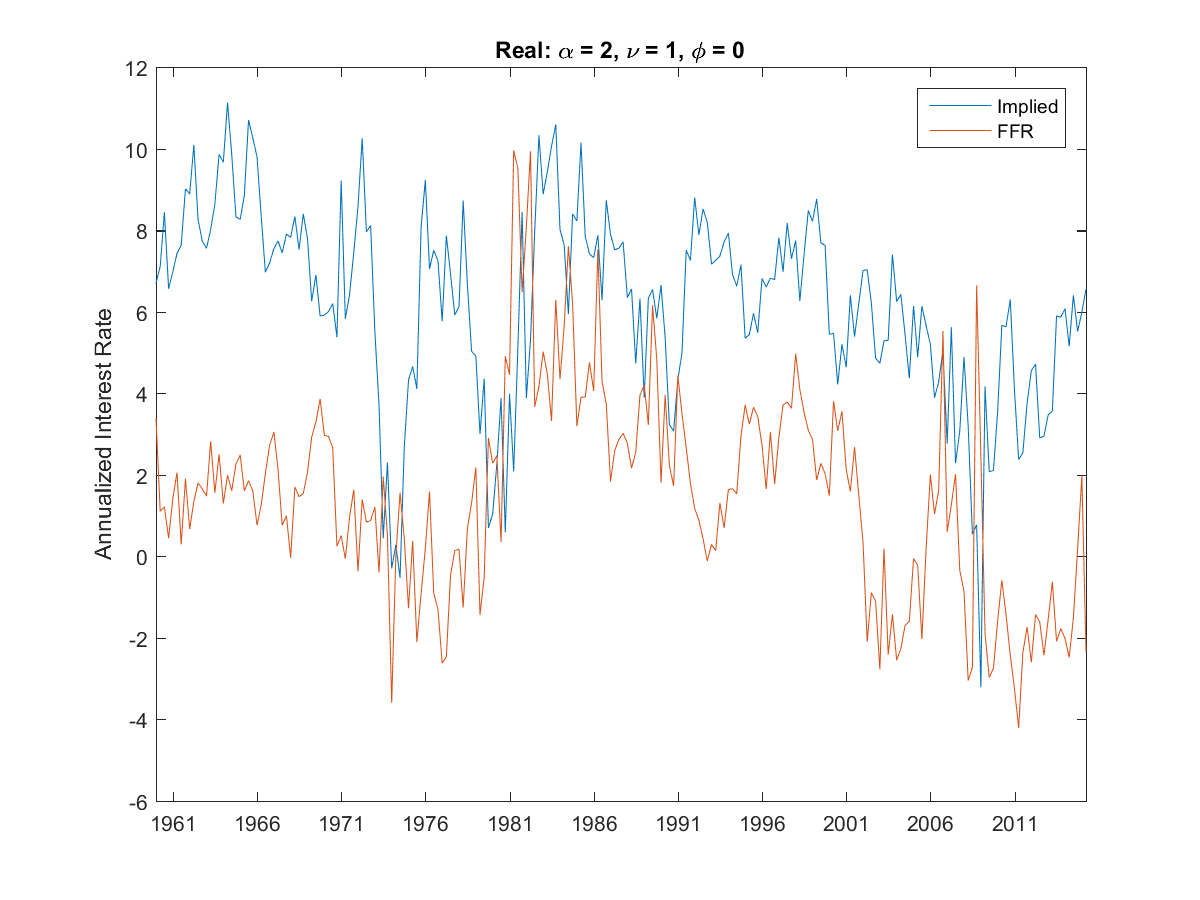
\includegraphics[width=0.49\textwidth]{figs/nipa/implied-vs-ffr/real_sep} &
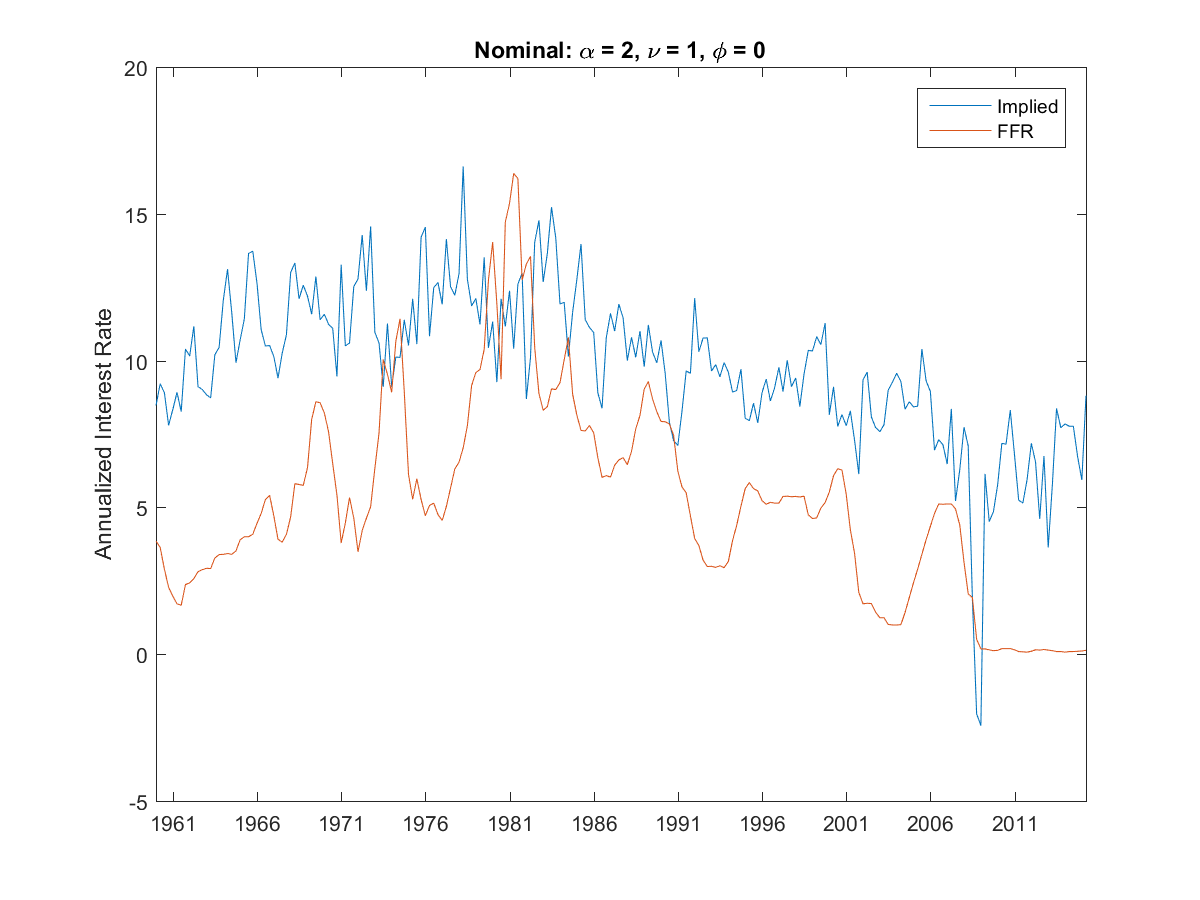
\includegraphics[width=0.49\textwidth]{figs/nipa/implied-vs-ffr/nominal_sep}
\end{tabular}
\caption{SEP implied vs. observed rates}
\label{implied-vs-ffr-nipa-sep}
\end{figure}



\subsection{Correlation of implied and observed rates}
Summary statistics for the implied rates under each specification are reported below in \autoref{implied-vs-ffr-nipa}, as well as the correlation between each implied rate and the effective federal funds rate.

The main result that stands out is the presence of strong positive correlations overall, but especially for nominal rates in the specifications without habit formation. Notably, the correlation between the nominal rate implied by CRRA preferences (SEP) and the historical nominal effective federal funds rate is 0.52, while adding nonseparability in leisure (NSEP) increases this correlation to 0.707. In the utility models with habit formation (SEP + HP and NSEP + HP), the correlation is less positive for nominal rates and essentially zero for real rates. These findings seem very much at odds with the qualitative appearance of the observed and implied rates moving in opposite directions.

\begin{table}[t]
\centering
\caption{Summary statistics for nominal and real rates (annualized rates)}
\label{implied-vs-ffr-nipa}
\begin{tabular}{lccccc} \hline
& Data & SEP & SEP + HP & NSEP & NSEP + HP \\ \hline
\multicolumn{6}{c}{Real interest rates} \\ \hline
\csvreader[head to column names, late after line = \\]%
  {tables/nipa/real.csv}{}%
  {\stat & \data & \sep & \sephp & \nsep & \nsephp} \hline
\multicolumn{6}{c}{Nominal interest rates} \\ \hline
\csvreader[head to column names, late after line = \\]%
  {tables/nipa/nominal.csv}{}%
  {\stat & \data & \sep & \sephp & \nsep & \nsephp} \hline
\end{tabular}
\end{table}

These strong positive correlations are noticeably higher than the still-positive correlations found by Collard and Dellas, to say nothing of the strongly negative values found by \cite{canzoneri07}. As a check, I reestimate the VAR and recompute the implied rates and correlations using only the time period spanned by Collard and Dellas, stopping at 2006:IV instead of 2015:II. The correlations for nominal rates from this restricted sample more closely resemble their results, though the ones for real rates are still rather different. I summarize the restricted sample results in \autoref{implied-vs-ffr-nipa-collard} in the appendix. In \autoref{correlation-comparison-nipa}, I compare the full and restricted sample correlations to those found in the other two papers. Note that the CCD paper examines several utility specifications, including CRRA (SEP) and Fuhrer habit preferences (SEP + HP), but does not include analysis of nonseparability in leisure.

\begin{table}[t]
\centering
\caption{Comparison of correlations between implied rates and effective FFR}
\label{correlation-comparison-nipa}
\begin{tabular}{lcccccc} \hline
                   & SEP   & SEP + HP & NSEP  & NSEP + HP & Start  & End \\ \hline
\multicolumn{7}{c}{Real interest rate correlation} \\ \hline
Full Sample        & 0.197 & -0.050   & 0.261 & 0.033     & 1960:I & 2015:II \\
Restricted Sample  & 0.020 & -0.098   & 0.065 & -0.058    & 1960:I & 2006:IV \\
\cite{collard11}   & 0.05  & 0.15     & 0.28  & 0.27      & 1960:I & 2006:IV \\
\cite{canzoneri07} & -0.37 & -0.07    & ---   & ---       & 1966:I & 2003:IV \\ \hline
\multicolumn{7}{c}{Nominal interest rate correlation} \\ \hline
Full Sample        & 0.520 & 0.142    & 0.707 & 0.390     & 1960:I & 2015:II \\
Restricted Sample  & 0.255 & 0.030    & 0.563 & -0.225    & 1960:I & 2006:IV \\
\cite{collard11}   & 0.26  & 0.04     & 0.63  & 0.38      & 1960:I & 2006:IV \\
\cite{canzoneri07} & 0.20  & -0.10    & ---   & ---       & 1966:I & 2003:IV \\ \hline
\end{tabular}
\end{table}

The extreme variation in correlations found suggests two points at which this analysis is not sufficiently robust.

First, comparing the correlations computed from the full sample to those from the restricted sample highlights the impact of the inclusion of the additional quarters from 2007:I to 2015:II. Scatter plots for both samples are shown in \autoref{nipa-full-vs-restricted-scatter}. (In particular, the data points in the restricted sample plot are not a subset of those in the full sample plot because the implied rates for each were computed using different VAR estimates.) The difference between the two samples is of course the era of near-zero interest rates following the Great Recession in 2008, which can be seen in the full sample plot as the cluster of observations on the FFR = 0 line. These, along with the outliers in the bottom left (which are also at the zero lower bound), drive the more strongly positive correlation in the full sample.

\begin{figure}[t]
\centering
\begin{tabular}{cc}
Full sample ($\rho = 0.520$) & Restricted sample ($\rho = 0.255$) \\
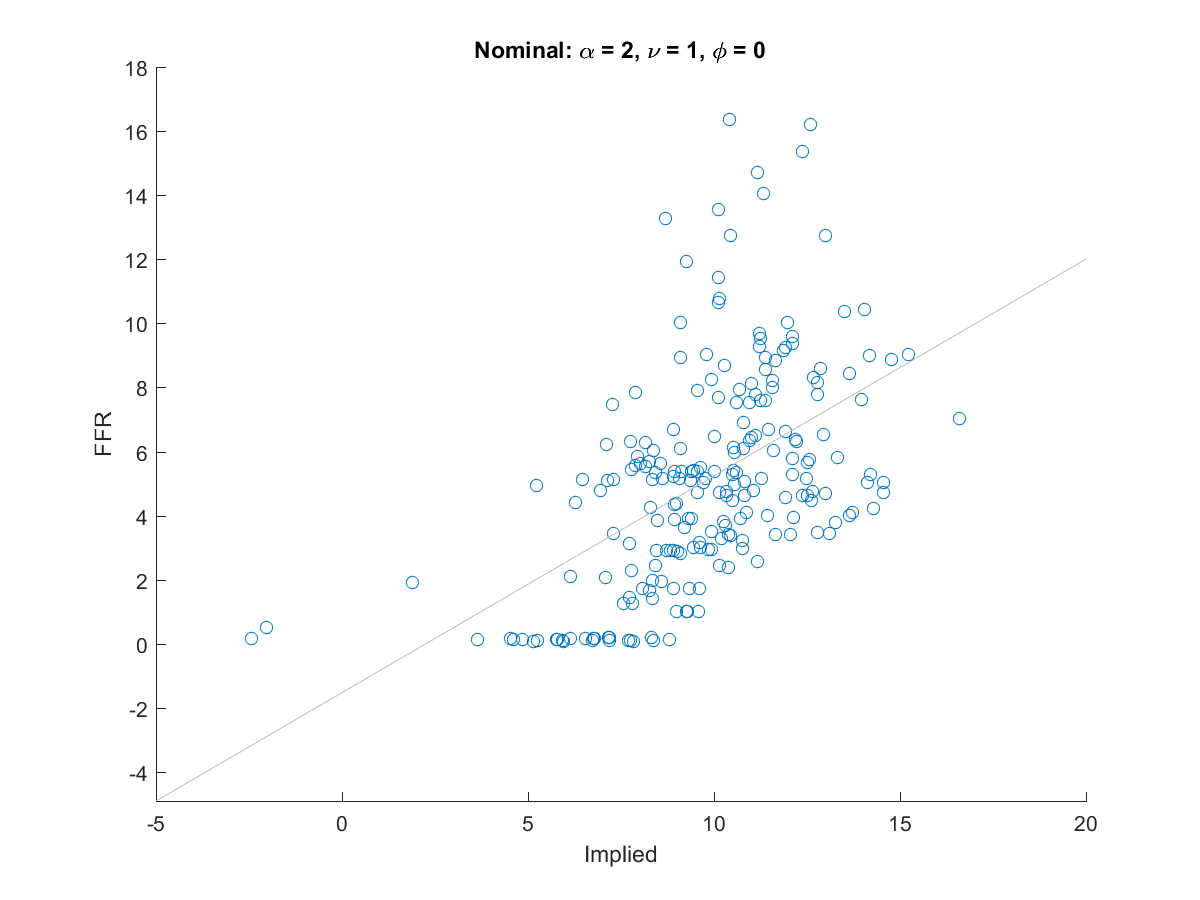
\includegraphics[width=0.49\textwidth]{figs/nipa/scatter/nominal_sep} &
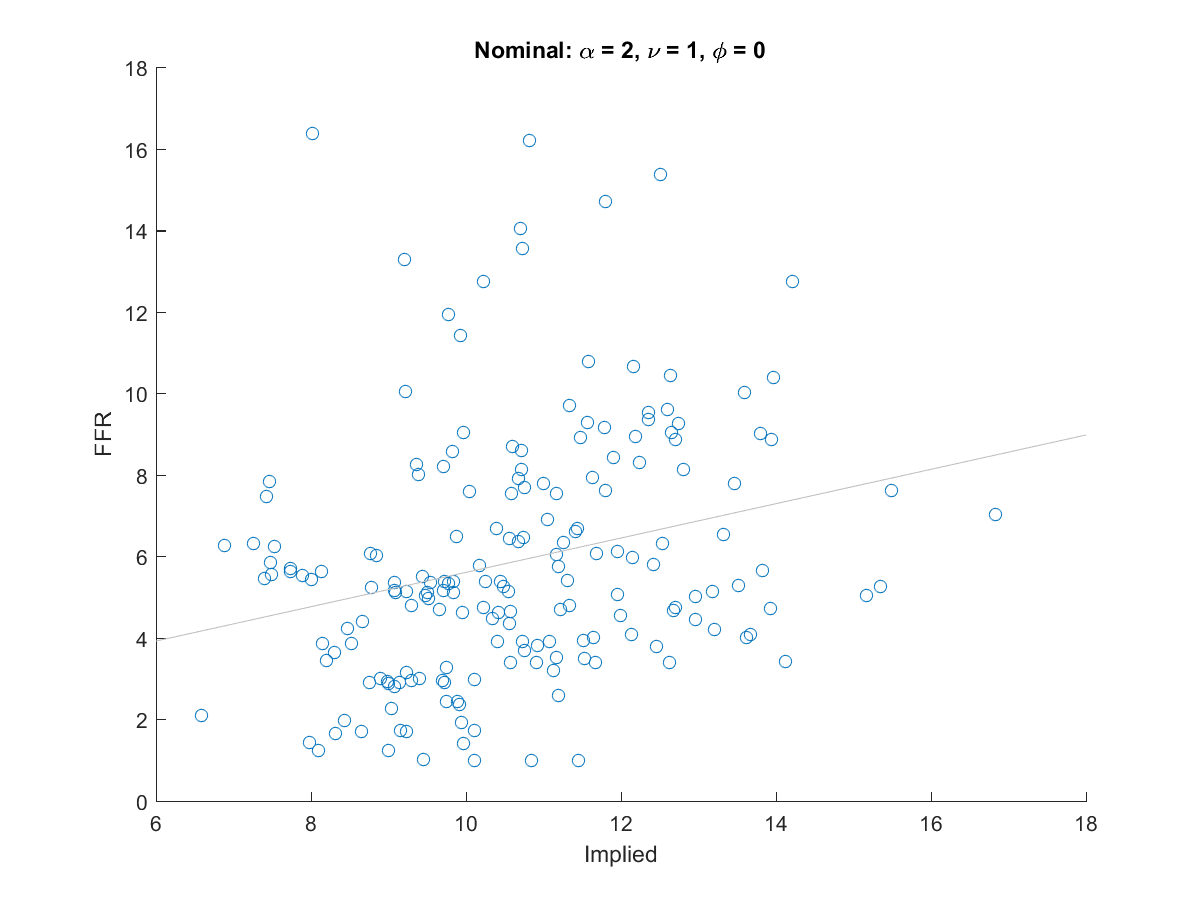
\includegraphics[width=0.49\textwidth]{figs/nipa/scatter/nominal_sep_collard} \\
\end{tabular}
\caption{SEP implied vs. observed nominal rates}
\label{nipa-full-vs-restricted-scatter}
\end{figure}

Even within the same time span, comparing the restricted sample correlations to those of Collard and Dellas highlights the fragility of these results with respect to small changes in methodology. I follow their specifications as closely as possible, except where it is not possible or not completely clear what they did. As mentioned in the previous section, due to lack of availability of data, I generate aggregate real consumption from the chain quantity indices scaled by the 2009 nominal consumption, while they use real consumption directly. I also estimate the VARs using log of gross quarterly inflation and interest rates $\pi_t$ and $ffr_t$, while it is possible that Collard and Dellas may have used annualized rates and/or scaled them to units of percentage points. Other possible differences include our choices of base year (2009 in my analysis, versus 2000) and whether we take the natural log of real dollars (as I do) or billions of real dollars.

All of this is to say that the correlation between the implied and observed rates is probably not the most reliable metric by which we should judge the fit of the consumption Euler equation to the data --- even though it's arguably the focus of both of these previous papers. A more consistent metric of fit is the correlation of the spread with the stance of monetary policy, which I discuss next.



\subsection{Response of spread to monetary policy}
It is clear that the implied and observed rates differ in level. In \autoref{implied-vs-ffr-nipa}, we see that the mean implied interest rate in each of the four utility specifications is noticeably higher than the mean ex post rate, in both the real and nominal cases. The lowest mean implied rates come from the full NSEP + HP utility model, with averages of 4.72 and 8.33 for the real and nominal rates respectively, compared to averages of 1.50 and 5.11 observed in the data in the same span.

If the model implied interest rates differed from the observed rates only by a constant factor, this discrepancy would be less worrisome. In practice --- for example, in larger macroeconomic models where the interest rate is assumed to be given by the Euler equation --- it would be easy to adjust for this constant ``measurement error''. However, as I show, and as CCD also find, this spread is in fact not constant, but correlated with the stance of monetary policy. In this aspect, my results strongly resemble those of CCD, as well as what one might expect from visually inspecting the plot of observed and implied rates.

I define the spread as the model implied interest rate less the observed rate. For each of the four utility specifications, I regress the spread on the effective (nominal) federal funds rate, as well as on four lags of itself. That is, I estimate using least squares the linear model
\begin{equation}
\label{spread-ffr-regression}
\mathrm{spread}_t = b_0 + b_1 \mathrm{FFR}_t + \sum_{j=1}^4 a_j \mathrm{spread}_{t-j}
\end{equation}
where all rates are annualized and given in units of percentage points. The estimated coefficients and standard errors for the federal funds rate only are reported below in \autoref{nipa-spread}. The FFR coefficients $b_1$ are negative for both real and nominal spreads under all four utility specifications. They are all significant at below the 1 percent level. This suggests that the difference between implied and observed rates tends to increase during periods of monetary expansion (lower FFR) and decrease during periods of monetary tightening.

\begin{table}[t]
\centering
\caption{Response of spread to nominal FFR}
\label{nipa-spread}
\begin{tabular}{lcccc} \hline
& SEP & SEP + HP & NSEP & NSEP + HP \\ \hline
\multicolumn{5}{c}{Real interest rates} \\ \hline
\csvreader[head to column names, late after line = \\]%
  {tables/nipa/spread-real.csv}{}%
  {\stat & \sep & \sephp & \nsep & \nsephp} \hline
\multicolumn{5}{c}{Nominal interest rates} \\ \hline
\csvreader[head to column names, late after line = \\]%
  {tables/nipa/spread-nominal.csv}{}%
  {\stat & \sep & \sephp & \nsep & \nsephp} \hline
\end{tabular}
\end{table}

These $b_1$ estimates match the negative coefficients estimated by CCD in direction, and are similar in magnitude. I also repeat this regression analysis using VAR estimates and implied interest rates generated using a restricted sample from 1966:I to 2003:IV, the time range used in their paper. I compare the estimates from the full and restricted samples to CCD in \autoref{spread-comparison-nipa} in the appendix.

Unlike the correlation between implied and observed rates, the results of regressing spread on the FFR do not change drastically in using this reduced sample, though they do resemble the CCD estimates slightly more than the full sample, as one might expect. This suggests that the response of the implied-observed spread to the FFR is a more robust instrument with which to measure the fit of the implied rate to the ex post rate than the correlation alone. It is also evidence that Collard and Dellas's addition of nonseparability in consumption and leisure to the CRRA model does not in fact improve the fit of the model implied rates to the data. While adding nonseparability does increase the correlation in models both with and without habit formation, it has little discernible effect on the estimated coefficient $b_1$.

As CCD discuss, these results indicate that something fundamental is not being captured by the consumption Euler equation, which leads to a difference between implied and observed rates that is not constant but systematically correlated with the stance of monetary policy. They also suggest an explanation for the divergence of the two series: from \eqref{nominal-euler-crra}, we see that the Euler equation implied rate increases in expected consumption growth. Expected consumption growth has been shown empirically to increase in response to monetary expansion (lower FFR), causing the implied rate to increase as well --- the opposite direction of movement from the actual interest rate.

I check this hypothesis by computing the orthogonalized impulse response of the model implied rate to a monetary shock. I compare the responses of the SEP implied real interest rate and the real FFR in \autoref{nipa-irf-sep}. The dashed lines indicate the 95 percent confidence interval, estimated from 1000 bootstrap simulations using \cite{kilian98}'s bootstrap code.  The results under the other three specifications were nearly identical, as were all of the nominal rate responses. As anticipated, a negative shock to real FFR causes a positive response in the model implied rate.

\begin{figure}[h]
\centering
\begin{tabular}{cc}
Real FFR & SEP Implied Real Rate \\
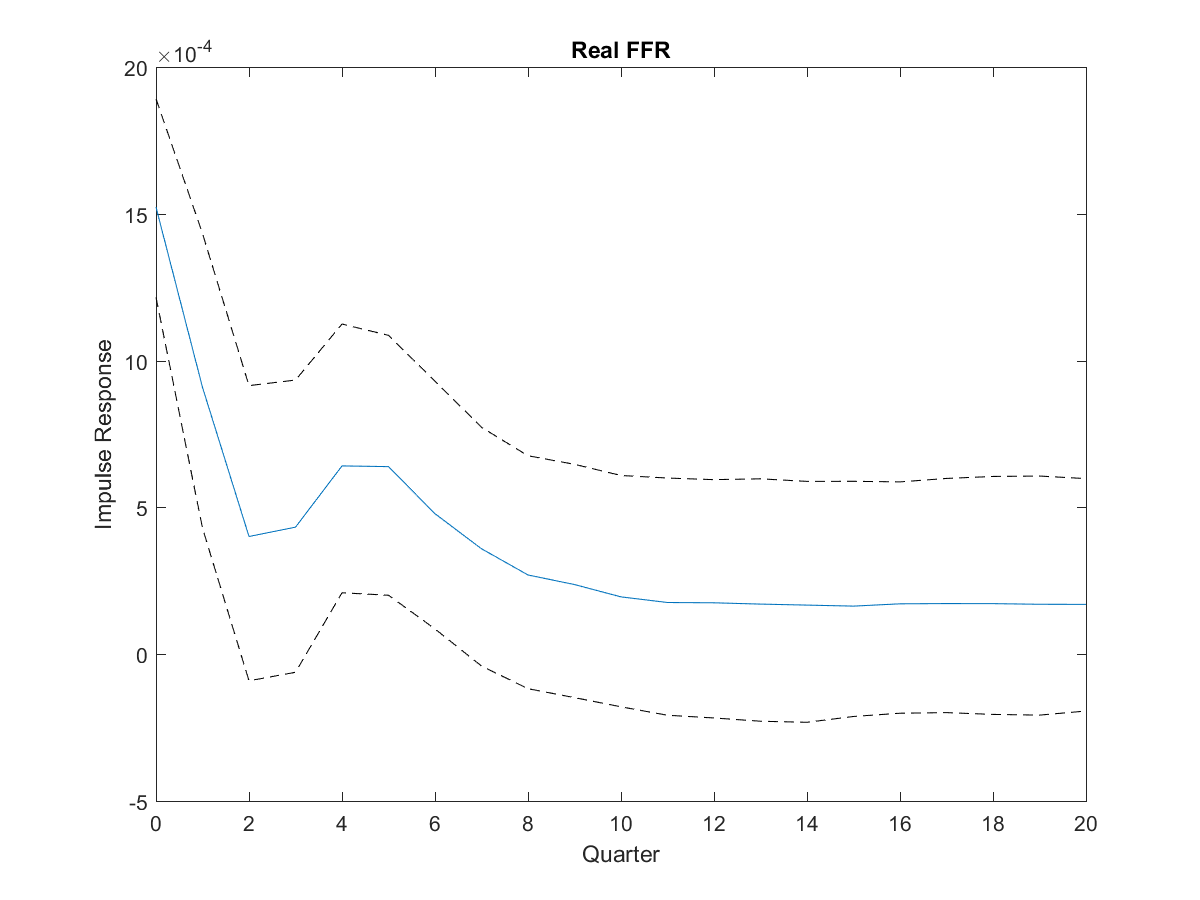
\includegraphics[width=0.49\textwidth]{figs/nipa/irf/real_ffr} &
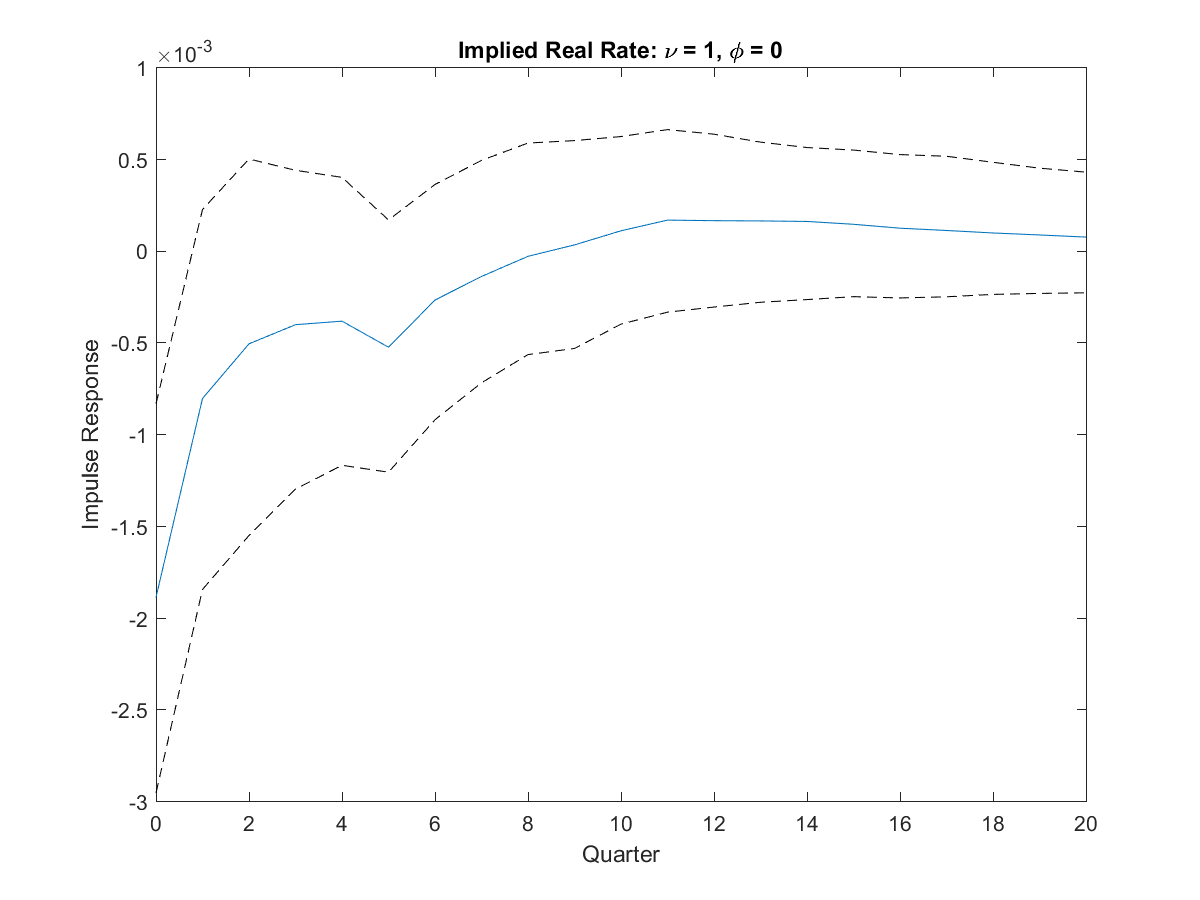
\includegraphics[width=0.49\textwidth]{figs/nipa/irf/real_implied_sep}
\end{tabular}
\caption{Impulse response to a monetary policy shock}
\label{nipa-irf-sep}
\end{figure}

Overall, it seems that despite the strong positive correlations between observed and implied rates that I find in each specification of utility, the path of the Euler equation implied interest rate, computed in this way, still deviates remarkably from the path of ex post rates. The addition of nonseparability in consumption and leisure that Collard and Dellas introduce does not change the implied rate's positive impulse response to the monetary policy shock, so by extension it also doesn't improve the estimated negative FFR coefficient in the spread regression \eqref{spread-ffr-regression}.